\lecture{2}{2021-09-01}{The grammar}

\section{`The grammar'}

\emph{Grammar} in linguistics is what we call \emph{descriptive}, not \emph{prescriptive}. That means if a sentence would be naturally said by a speaker of a language, the sentence is considered \emph{grammatical} for our data. This includes:

\ex. What should I talk about? (Ending a sentence with a proposition happens all the time in speech.)

\ex. Who is this for? (Using `who' where you might have been taught to use `whom'.)

Judgments about grammaticality are usually innate. That means you can judge if a word or sentence ``sounds good'' in your language without any formal education or training.
You don't need to know how to read or write to have linguistic judgments.
In fact, very young children also have intuitions about language.

\subsection{The Wug Test}

\begin{figure}[htbp]
	\centering
	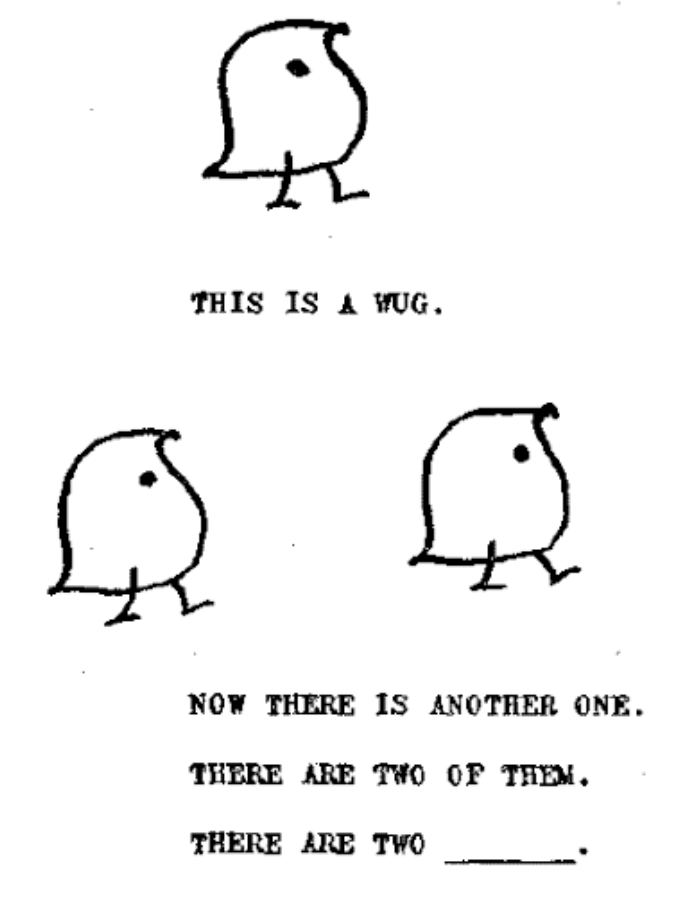
\includegraphics[width=.3\textwidth]{wug_test}
	\caption{The Wug Test (Berko, 1958)}
\end{figure}

The Wug test is checking the ability to generate a regular plural --- which is the suffix (-s) in English --- so this is in the realm of morphology and not necessarily syntax --- although there is a gray area between morphology and syntax, since how we define a single `word' is not super clear.

However, language users have intuitions in all areas of the grammar --- which will serve as a handy overview of generative linguistics.

\underline{Aside:} What is generative linguistics? This is a particular approach to studying language which assumes humans have a \emph{generative capacity}, i.e., the ability to generate linguistic forms, using some internal set of rules. This is often contrasted with \emph{funcionalist} approaches, which care more about the function of linguistic elements rather than the generative algorithm or set of rules used to produce them. These two approaches are actually compatible in most cases, but many colleges/linguists fall into one ``camp'' and might malign the other --- if they think about them at all. We will be looking at things through a generative lens in this class, but that doesn't mean it's the only way! 

\section{Areas of Linguistics}

\paragraph{Phonology.} The study of sound patters --- or patters in parameters of signs, for signed languages.

\ex. blick

\ex. ?bnick

\ex. *bfick

\paragraph{Morphology.} The study of word-internal structure --- like prefixes, suffixes, in-freakin'-fixes, etc. Not so different from syntax.

\ex. run

\ex. runs

\ex. run-(n)er

\ex. *run-s-er

\paragraph{Syntax.} The study of sentence structure --- like nouns, verbs, etc. More on this later.

\paragraph{Semantics.} The study of meaning as encoded in language.

\ex. I just stopped smoking. Now my lungs are feeling fresh.

\ex. I just stopped smoking. \#But in fact, I have never smoked.

\ex. \#This jar is green and not a jar.

\paragraph{Pragmatics.} The study of meaning in contex --- social context, language context, cultural context.

\ex. \emph{Don't tell your friends about your indigestion, ``how are you?'' is a greeting, not a question.}

\paragraph{Others.} Of course there are many other `named' areas of study in linguistics: socioling, anthroling, acquisition, compling, neuroling, psycholing, internet ling, phonetics, conversation analysis, philosophy of language, etc. --- but they are often overlapping/combined with the study of those various areas of the grammar listed above.

\chapter{Syntax}

Syntax is about how sentences are put together. In other to actually talk about the structure of a sentence, we need some categories, because there are too many words to list out individual rules. For example:

\begin{enumerate}[label = \textbullet, itemsep = 2pt]
	\item {[Noun Verb]} makes a fine sentence.
		
		\ex. Cats talk.

		\ex. Cats walk.

		\ex. Dogs talk.

		\ex. Dogs walk.

	\item But [Verb Noun] doesn't really (unless these are commands).

		\ex. *Talk cats.

		\ex. *Walk cats.

		\ex. *Talk dogs.

		\ex. *Walk dogs.

\end{enumerate}

So rather than listing \(\{\text{Cats}, \text{Dogs}, \dots\} + \{\text{Walk}, \text{Talk}, \dots\} = \text{English sentence}\), we can use the shorthands ``Noun'' and ``Verb''.





